\documentclass[crop,class=article]{standalone}
%----------------------------Preamble-------------------------------%
\usepackage{tikz}
%--------------------------Main Document----------------------------%
\begin{document}
    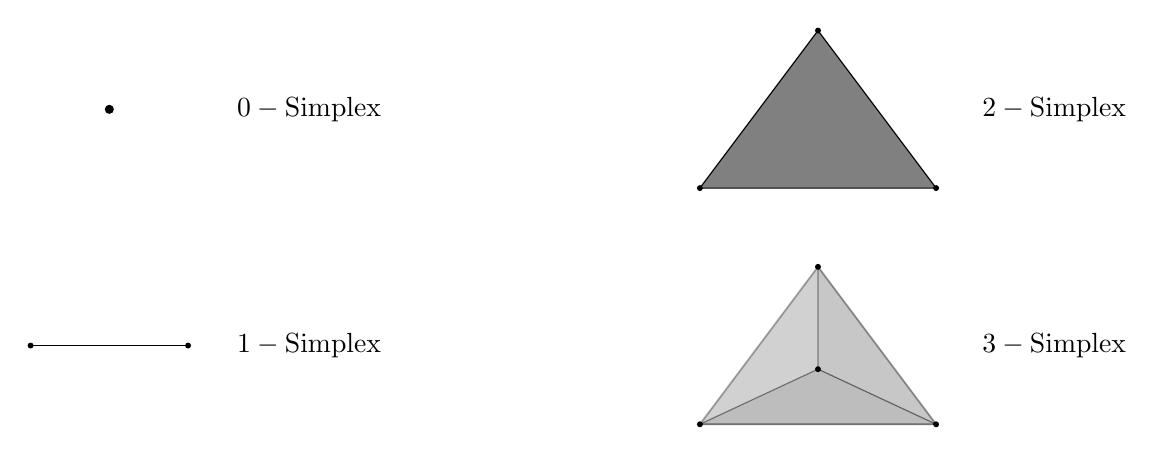
\begin{tikzpicture}
        \node at (1.5,1) [right] {$0-\textrm{Simplex}$};
        \node at (1.5,-2) [right] {$1-\textrm{Simplex}$};
        \node at (12,1) {$2-\textrm{Simplex}$};
        \node at (12,-2) {$3-\textrm{Simplex}$};
        \draw[fill=black] (0,1) circle (0.05);
        \draw[fill=black] (-1,-2) circle (0.03);
        \draw[fill=black] (1,-2) circle (0.03);
        \draw[draw=black] (1,-2) -- (-1,-2);
        \draw[fill=gray] (9,2)--(7.5,0)--(10.5,0)--cycle;
        \draw[fill=black] (9,2) circle (0.03);
        \draw[fill=black] (7.5,0) circle (0.03);
        \draw[fill=black] (10.5,0) circle (0.03);
        \draw[fill=gray,opacity=0.2]
            (9,-1)--(7.5,-3)--(9,-2.3)--cycle;
        \draw[fill=gray,opacity=0.3]
            (9,-1)--(10.5,-3)--(9,-2.3)--cycle;
        \draw[fill=gray,opacity=0.4]
            (9,-2.3)--(7.5,-3)--(10.5,-3)--cycle;
        \draw[fill=gray,opacity=0.2, thick]
            (9,-1)--(7.5,-3)--(10.5,-3)--cycle;
        \draw[fill=black] (9,-1) circle (0.03);
        \draw[fill=black] (7.5,-3) circle (0.03);
        \draw[fill=black] (10.5,-3) circle (0.03);
        \draw[fill=black] (9,-2.3) circle (0.03);
    \end{tikzpicture}
\end{document}